
\documentclass{article}
\usepackage[english]{babel}
\usepackage[T1]{fontenc}
\usepackage[utf8]{inputenc} 
\usepackage{times}
\usepackage{amsfonts}

\usepackage{mathtools, bm}
\usepackage{amssymb, bm}	
\usepackage{tikz,tkz-tab}
\usepackage{subcaption}

\usepackage{booktabs}

\usepackage[]{algorithm2e}
\usepackage{enumerate}
\usepackage{amsmath}
\usepackage{graphicx}
\usepackage[colorinlistoftodos]{todonotes}
\usepackage{hyperref}
\usepackage{tabularx}
\usepackage{listings}


\usepackage{amsmath}
\DeclareMathOperator*{\argmax}{arg\,max}
\DeclareMathOperator*{\argmin}{arg\,min}

\title{TP 2: Semi-supervised learning (SSL)}
\author{Raphaël Chekroun}
\date{}

\usepackage[a4paper,top=3cm,bottom=2cm,left=3cm,right=3cm,marginparwidth=1.75cm]{geometry}


\begin{document}

\maketitle
\section{Question 1}


1. With the information of only 4 random labels and a 6-nn graph, we get an accuracy of 100\% (with some luck on the choice of the labels, I guess):
\begin{center}
	\includegraphics[scale=0.7]{1}
\end{center}

Note that I used the closed form solution from class which is 
$$
f_u = L_{uu}^{-1} W_{ul}f_l
$$

2. With the larger two moon dataset, with a 6-nn graph and 4 random labels, the accuracy is still of 100\%.
The image is the same but more "dense":
\begin{center}
	\includegraphics[scale=0.7]{2}
\end{center}

3. We have the optimization problem:
$$
min_f (f-y)^T C (f-y) + 2f^T L
$$
Let's compute a closed form solution by canceling the Lagrangian to get:
$$
2\left((f-y)^T C + f^T L\right) = 0 \iff \boxed{f = \left(y^T C (L+C)^{-1}\right)^T}
$$
Thus we can compute the formula directly on Python. $f$ being of dimension $(num\_samples \times num\_classes)$, not any constraints is necessary and the label of each node will be the column maximizing the line.

After implementation, we get, for two\_moons using $c_u = c_l = 1$, an accuracy of 100\%:
\begin{center}
	\includegraphics[scale=0.7]{3}
\end{center}


Once this has been done, I completed hard\_vs\_soft\_hfs and got the following results:
\begin{center}
	\includegraphics[scale=0.7]{4}
\end{center}
The accuracy was of 92.5\% for Hard-HFS and 98.5\% for Soft-HFS.

Of course, I did the test several times, as the wrong labels are random, and the results are always close to this. We notice that the results seems to always be better for Soft-HFS. It depended a lot of $c_u$ and $c_l$ parameter, and after some fune-tuning I found the parameters $c_u=0.05$ and $c_l=0.95$ to be the best on this dataset. 

\section{Question 2}


To complete the code, I added the piece of code allowing to sort X and Y according to Y, in order to have all the unlabeled together, thus knowing where is what we called in class $L_{uu}$ (submatrix of unlabeled nodes of the Laplacian). I also gave the parameters the needed values, as before.

With Soft-HFS, a 6-nn graph and $c_l=0.95$ and $c_u=0.05$, the best accuracy reached was of $87\%$ (see next figure). 
With Hard-HFS I managed to make it reach only $81\%$ with the same parameters, chosing a very big gamma (100) to avoid having $L_{uu}$ has a singular matrix.

\begin{center}
	\includegraphics[scale=0.7]{5}
\end{center}

1. In order to label more than two classes, I implented all my vectors as one-hot vectors of dimensions $(n \times num\_classes)$ and not just vectors of dimension $n$ containing binary information. It means that the target vector is $y \in \{0,1\}^K$.
\\ \newline 


2. I tried a lot a combination (with or without equalizeHist, with or without GaussianBlur, with or without BilateralFilter, with or without blur). I also try all the combinations of the previoulsy cited functions, after fune-tuning by applying each of them alone until I have the best accuracy for it, of 87\%. 

The best result overall was obtained with using only cv2.blur with a kernel of size $(50,50)$, for Soft-HFS with $c_l=0.95$ and $c_u=0.05$.

The best result for hard-HFS is $81\%$ and is also with blur with a kernel of size $(50,50)$.
\\ \newline 


3. HFS seems to be quiet efficient here (after all, $87\%$ seems good to me!). 

Nonetheless, we can't say anything realtively to what can be done as we didn't tested it on common datasets in order to compare it to state-of-the-art algorithms, sometimes reaching an accuracy of more than $99\%$ (according to "Deep Face Recognition: A Survey" by M. Wang, W. Deng).
\\ \newline 



4. Addind more data indeed increased the performance, as I was now able to obtain an accuracy of $98.8\%$, with the same parameters as the previous optimal results.
\begin{center}
	\includegraphics[scale=0.7]{6}
\end{center}

The accuracy is sensibly improved thanks to the amount of available labels data which is higher than before, thus giving the chance, after masking labels, to get a more uniformly distributed known label distribution on the graph, making the "propagation" of labels more robust.

\section{Question 3}
1. The function has been simply completed following the given pseudo-code.
\\ \newline

2. Same here, with the particularity that I had to implement a new function in harmonic\_function\_solution.py. It's a modification of hard\_HFS, called hard\_HFS\_ssl\_online. It's basically the same function but that don't take the same arguments (only L, W and Y) and don't return labels but f.
\\ \newline

3. The first thing to notice on my implementation is that I chose to make of $c\_add$ and $c\_rep$ not the centroids themselves, but their indexes.
After some work and modification of the given code, I achieved a working algorithm.


\begin{center}
	\includegraphics[scale=0.15]{0}
\end{center}

\begin{center}
	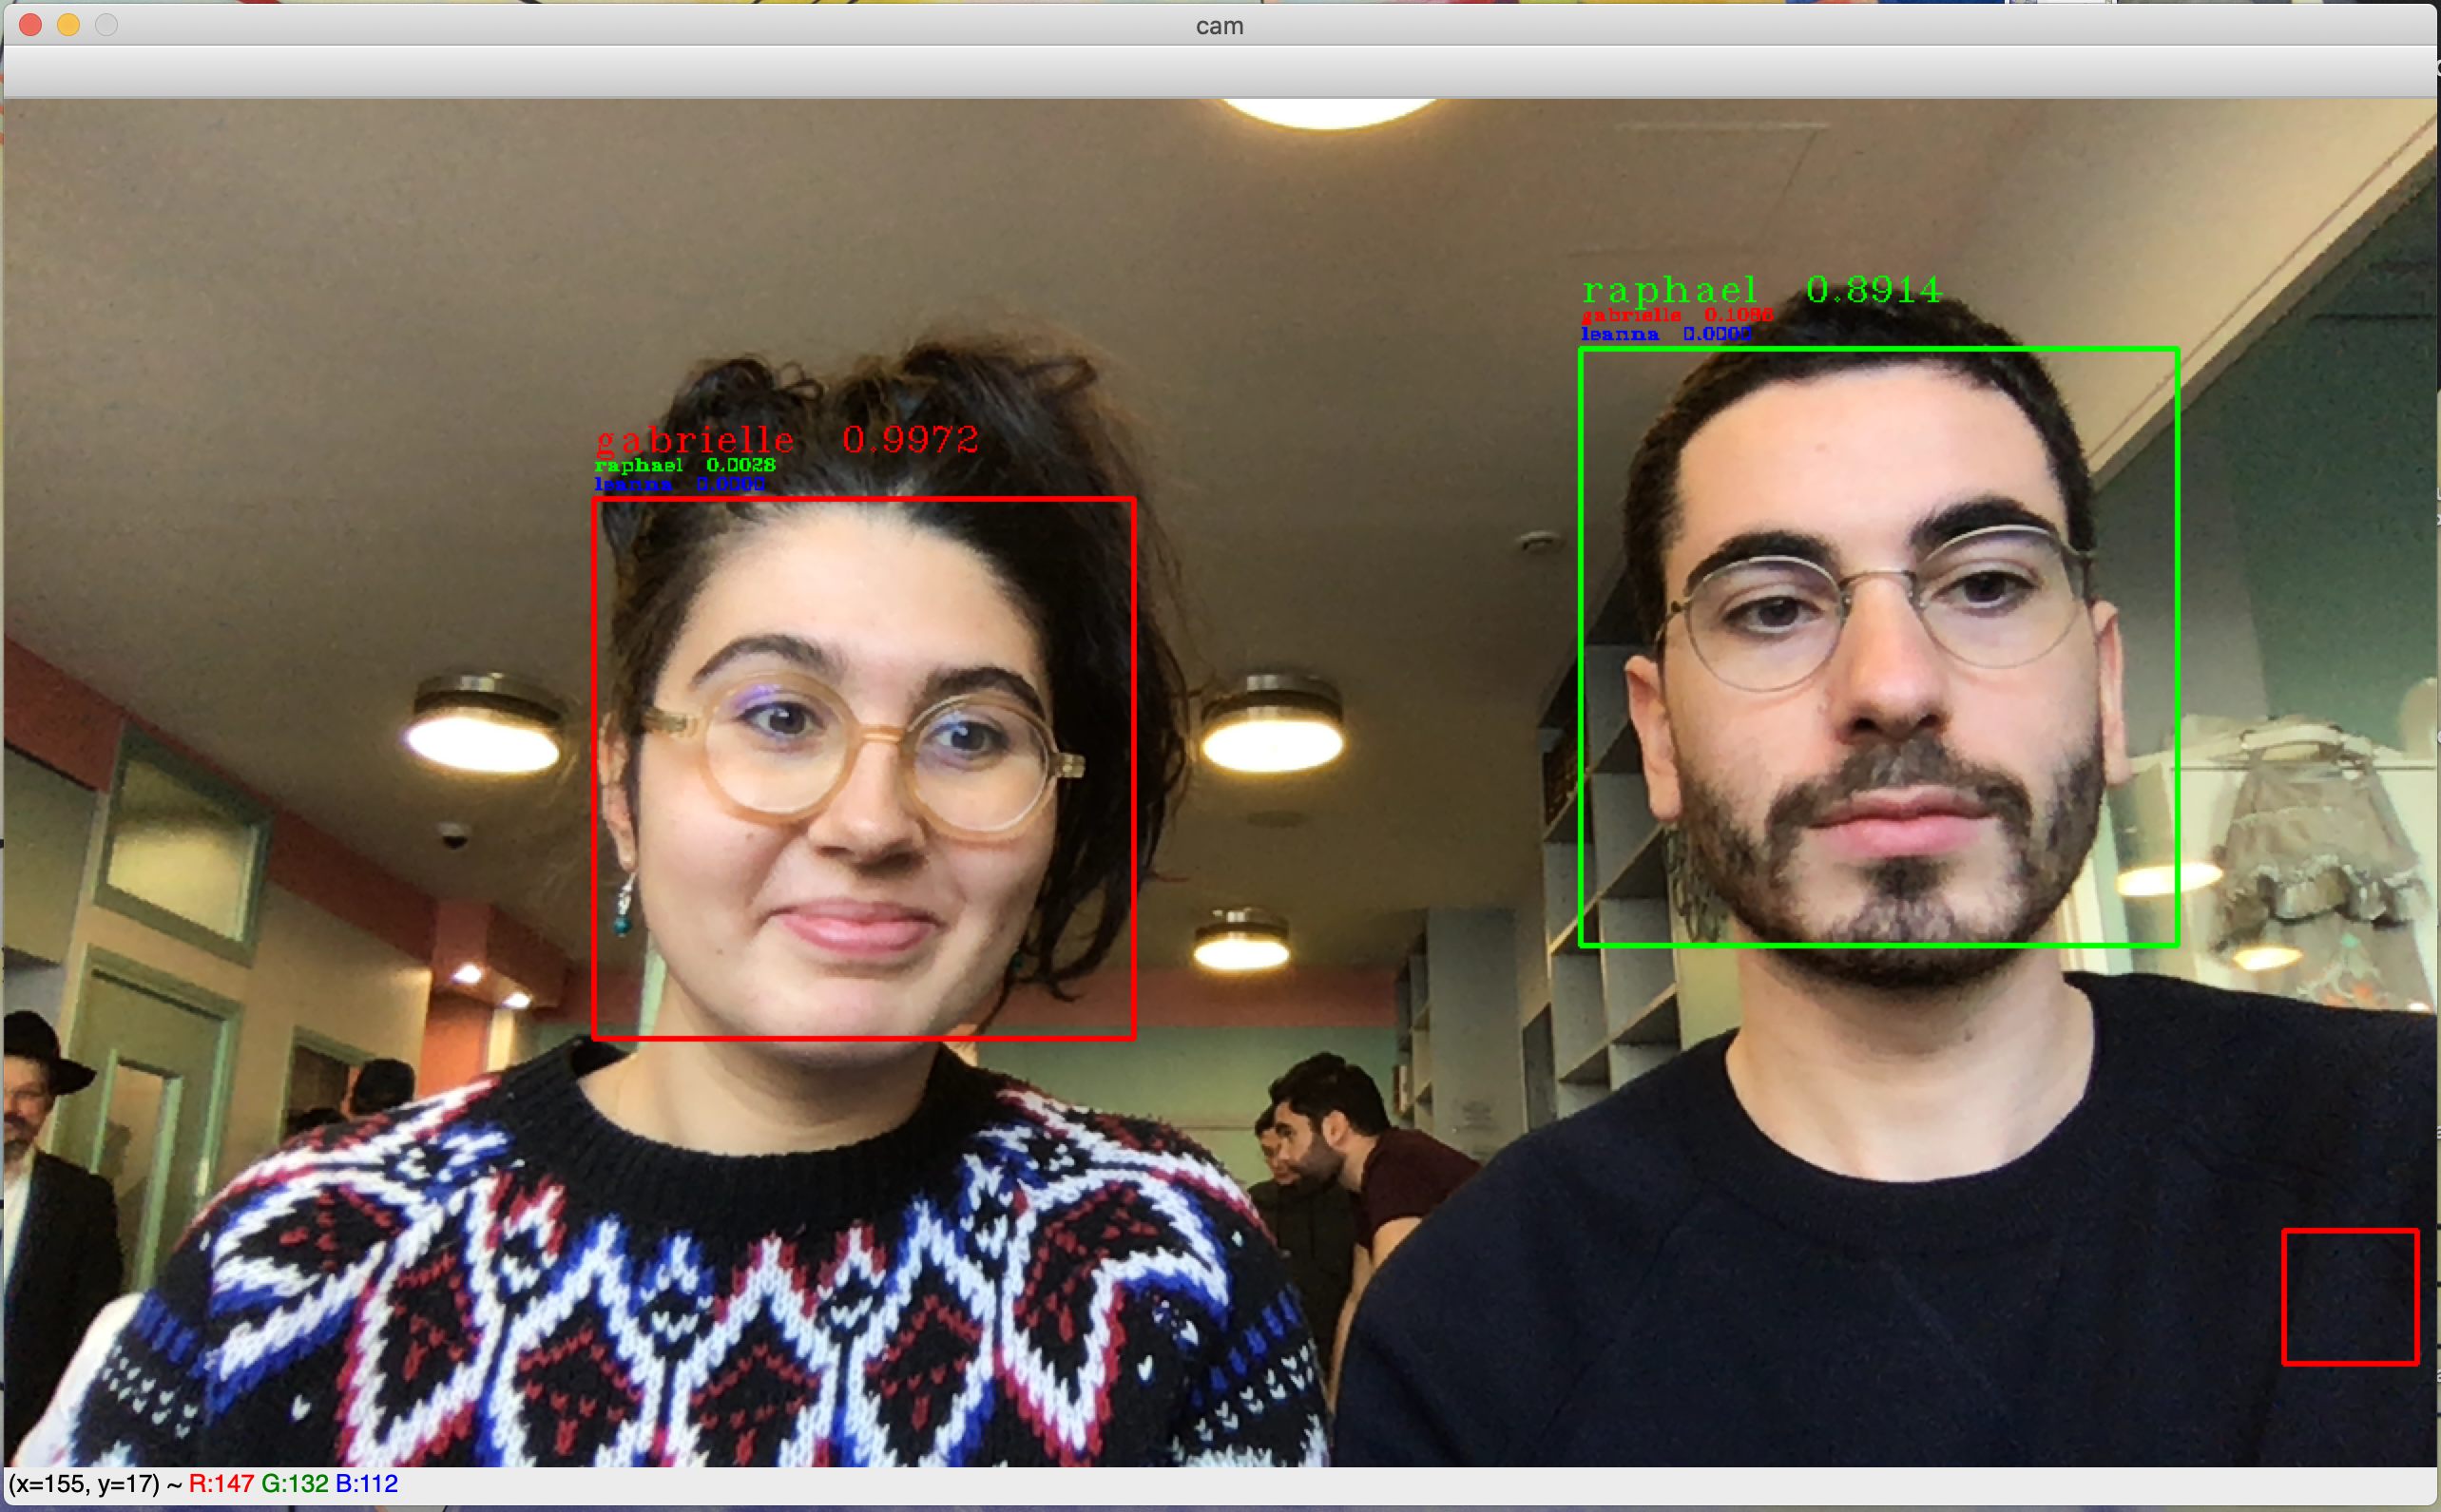
\includegraphics[scale=0.15]{7}
\end{center}

pour 
\end{document}